\section{Empirical Investigation}
\label{sec:experiments}

We empirically investigate three questions. First, can factual
predictive accuracy conceal failures in treatment-relevant latent
representation and temporal propagation? Second, does Temporal JEPA
improve long-horizon treatment-effect estimation while maintaining
factual predictive performance? Third, how sensitive are the observed
improvements to treatment timing, rollout horizon, training design, and
model-selection choices? We use a controlled longitudinal medical
system in which the complete observed history satisfies the assumed
causal identification conditions and the ground-truth treatment-effect
trajectory is available for evaluation. Full simulator equations, data
generation, model hyperparameters, and additional results are provided
in Appendix~\ref{app:experimental-details}.

\subsection{Experimental Setup}
\label{sec:experimental-setup}

\paragraph{Controlled medical dynamics.}
The system contains a primary clinical outcome $X_t$, a time-varying
clinical covariate and treatment-effect modifier $C_t$, decaying
cumulative treatment exposure $D_t$, lagged treatment $A_{t-1}$, and
an observed nuisance variable $U_t$. Treatment $A_t\in\{0,1\}$ is
assigned by a state-dependent historical policy. The outcome of
interest is $Y_t=X_t$, while the world model predicts the joint clinical
state $V_t=(X_t,C_t)$. The design deliberately combines four mechanisms:
effect modification through $C_t$, delayed response through $A_{t-1}$,
cumulative exposure through $D_t$, and persistent but causally
irrelevant variation through $U_t$. These mechanisms separately test
whether a learned latent state preserves treatment-relevant history,
propagates it through recursive transitions, and avoids allocating
limited capacity only to predictively salient information.

This simulator is not intended to reproduce a particular disease. It is
a mechanism-isolation environment designed to be stable, interpretable,
and sufficiently non-linear to distinguish ordinary trajectory fitting
from treatment-conditioned temporal simulation. All variables driving
treatment and outcome are observed, or deterministically recoverable
from the observed treatment history. Thus, the experiment isolates
finite-model realization error rather than non-identifiability caused
by unmeasured confounding. Exact equations and a component-by-component
design rationale are given in Appendix~\ref{app:simulator}.

\paragraph{Models and baselines.}
All models use the same two-layer Transformer history encoder,
action-conditioned residual latent transition, and outcome decoder.
Unless otherwise stated, the latent dimension is eight. We compare:
\begin{enumerate}
    \item \textbf{One-step prediction}, which supervises only
    $(X_{t+1},C_{t+1})$;
    \item \textbf{Multi-step prediction}, which recursively predicts
    $(X,C)$ for eight observed future transitions; and
    \item \textbf{Temporal JEPA}, which adds the action-conditioned
    multi-horizon latent objective at
    $\mathcal H_J=\{1,2,4,8\}$.
\end{enumerate}
The three methods use identical factual training trajectories. Temporal
JEPA does not use counterfactual trajectories or treatment-effect
targets during training. We train five random seeds per configuration.
Architecture and optimization details are in
Appendix~\ref{app:model-details}.

\paragraph{Evaluation schedules.}
Every effect evaluation starts from the same observed patient history
and contrasts a prespecified treatment schedule against no future
treatment. We consider a four-step early block, an alternating schedule,
a separated schedule with treatment at steps $\{0,4,8,12\}$, and a
late-separated schedule with treatment at steps $\{3,7,11,15\}$. The
last two schedules contain the same number of treatments and differ only
in timing. These schedules are not supplied as explicit training
policies; training uses trajectories sampled from the historical
state-dependent assignment mechanism. Because that mechanism is
stochastic, we do not claim that every local action pattern is absent
from training. Rather, the evaluation tests whether the learned
transition can compose locally observed state--action relationships
under prespecified temporal arrangements. Schedule definitions and the
counterfactual evaluation protocol are detailed in
Appendix~\ref{app:schedules}.

\paragraph{Metrics and selection.}
We report three complementary metrics. Observed rollout MSE measures
factual trajectory fidelity for $V_t=(X_t,C_t)$. Latent closure MSE
compares a recursively predicted future latent state with the state
obtained by directly re-encoding the corresponding observed future
history. Effect trajectory MSE evaluates the primary outcome $Y_t=X_t$:
\begin{equation}
    \mathcal R_{\mathrm{effect}}^{(H)}
    =
    \frac{1}{NH}
    \sum_{i=1}^{N}\sum_{h=1}^{H}
    \left(\widehat\tau_{i,h}-\tau_{i,h}\right)^2.
\end{equation}
Hyperparameters are selected using a separate observational validation
set only. We first retain JEPA configurations whose eight-step observed
rollout MSE is within $10\%$ of the multi-step prediction baseline, and
then select the eligible configuration with the lowest eight-step latent
closure MSE. No counterfactual metric enters this procedure. This rule
selects $\lambda_J=1$. Dataset splits and the complete selection rule are
given in Appendices~\ref{app:data-generation}
and~\ref{app:model-selection-details}.

\subsection{Diagnosing Failures in Latent World Models}
\label{sec:latent-diagnosis}

We first test the two failure mechanisms motivating our method:
information loss during history compression and incorrect use or
propagation of information already present in the latent state.

\subsubsection{Information Loss under Latent Compression}

We train factual multi-step world models with latent dimensions
$d_z\in\{1,2,4,8,16\}$, using five seeds for each dimension. After
training, the world model is frozen and simple linear probes measure
whether $X_t$, $C_t$, accumulated dose $D_t$, lagged treatment, and the
nuisance $U_t$ can be recovered from $Z_t$. These probes are diagnostic:
they do not modify the world model and are not used for model selection.

At $d_z=1$, current severity remains highly recoverable
($R^2=0.927$), whereas the treatment-effect modifier is largely lost
($R^2=0.073$). Its factual prediction MSE is only $2.6\%$ worse than
that of $d_z=2$, but its horizon-16 treatment-effect MSE is $2.55$
times larger. Increasing capacity makes $C_t$, dose, and lagged
treatment recoverable, but also increasingly encodes the causally
irrelevant nuisance. Moreover, larger states do not monotonically
improve effect estimation: $d_z=16$ achieves lower factual error than
$d_z=4$ but approximately twice its effect error. These results support
the existence of a representation gap, while also showing that capacity
alone is not a measure of intervention fidelity.

\begin{figure*}[t]
    \centering
    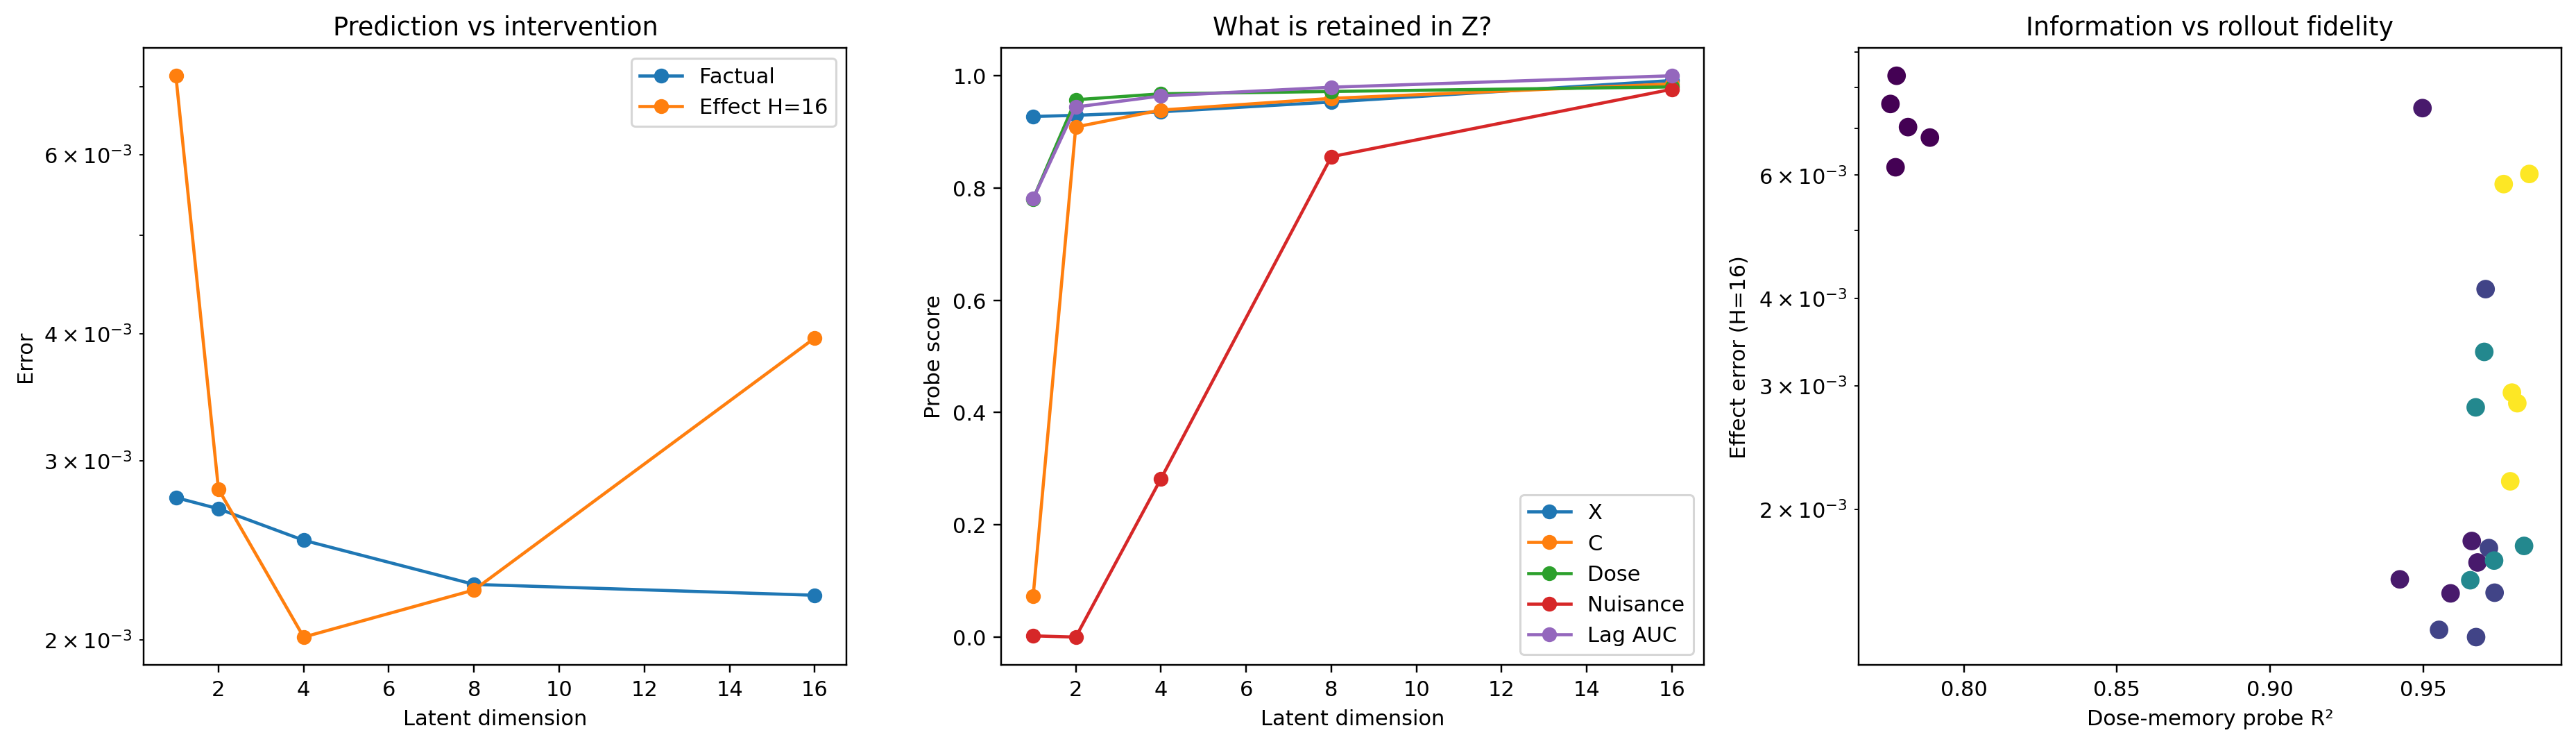
\includegraphics[width=0.97\textwidth]
    {figures/medical_latent/latent_information_diagnosis.png}
    \caption{Latent-capacity diagnosis. Limited capacity can preserve
    severity while losing the treatment-effect modifier; larger capacity
    recovers treatment-relevant variables but also encodes nuisance
    information and does not monotonically improve long-horizon effect
    estimation. Results aggregate five seeds per latent dimension.}
    \label{fig:latent-capacity}
\end{figure*}

\subsubsection{Failure to Propagate Retained Information}

Recoverability from the encoded state does not imply that the transition
uses the information correctly. To separate representation from
propagation, we compare two states at each future horizon: a rolled state
obtained by recursively applying the learned transition and an encoded
state obtained by applying the frozen encoder to the corresponding true
future history. We then evaluate the local treatment response implied by
each state. If encoded-state response error is small but rolled-state
error is large, the relevant information remains available in the
representation but has been corrupted by recursive transition.

Across 45 fitted world models spanning multiple latent capacities and
training objectives, the median rolled-to-encoded response-error
amplification at horizon 16 is $4.82$. In total, $68.9\%$ of models
exceed a factor of two and $48.9\%$ exceed a factor of five. Thus,
accurate local representation does not by itself guarantee stable
temporal propagation. Complete model-family definitions are provided in
Appendix~\ref{app:transition-diagnosis}.

\begin{figure*}[t]
    \centering
    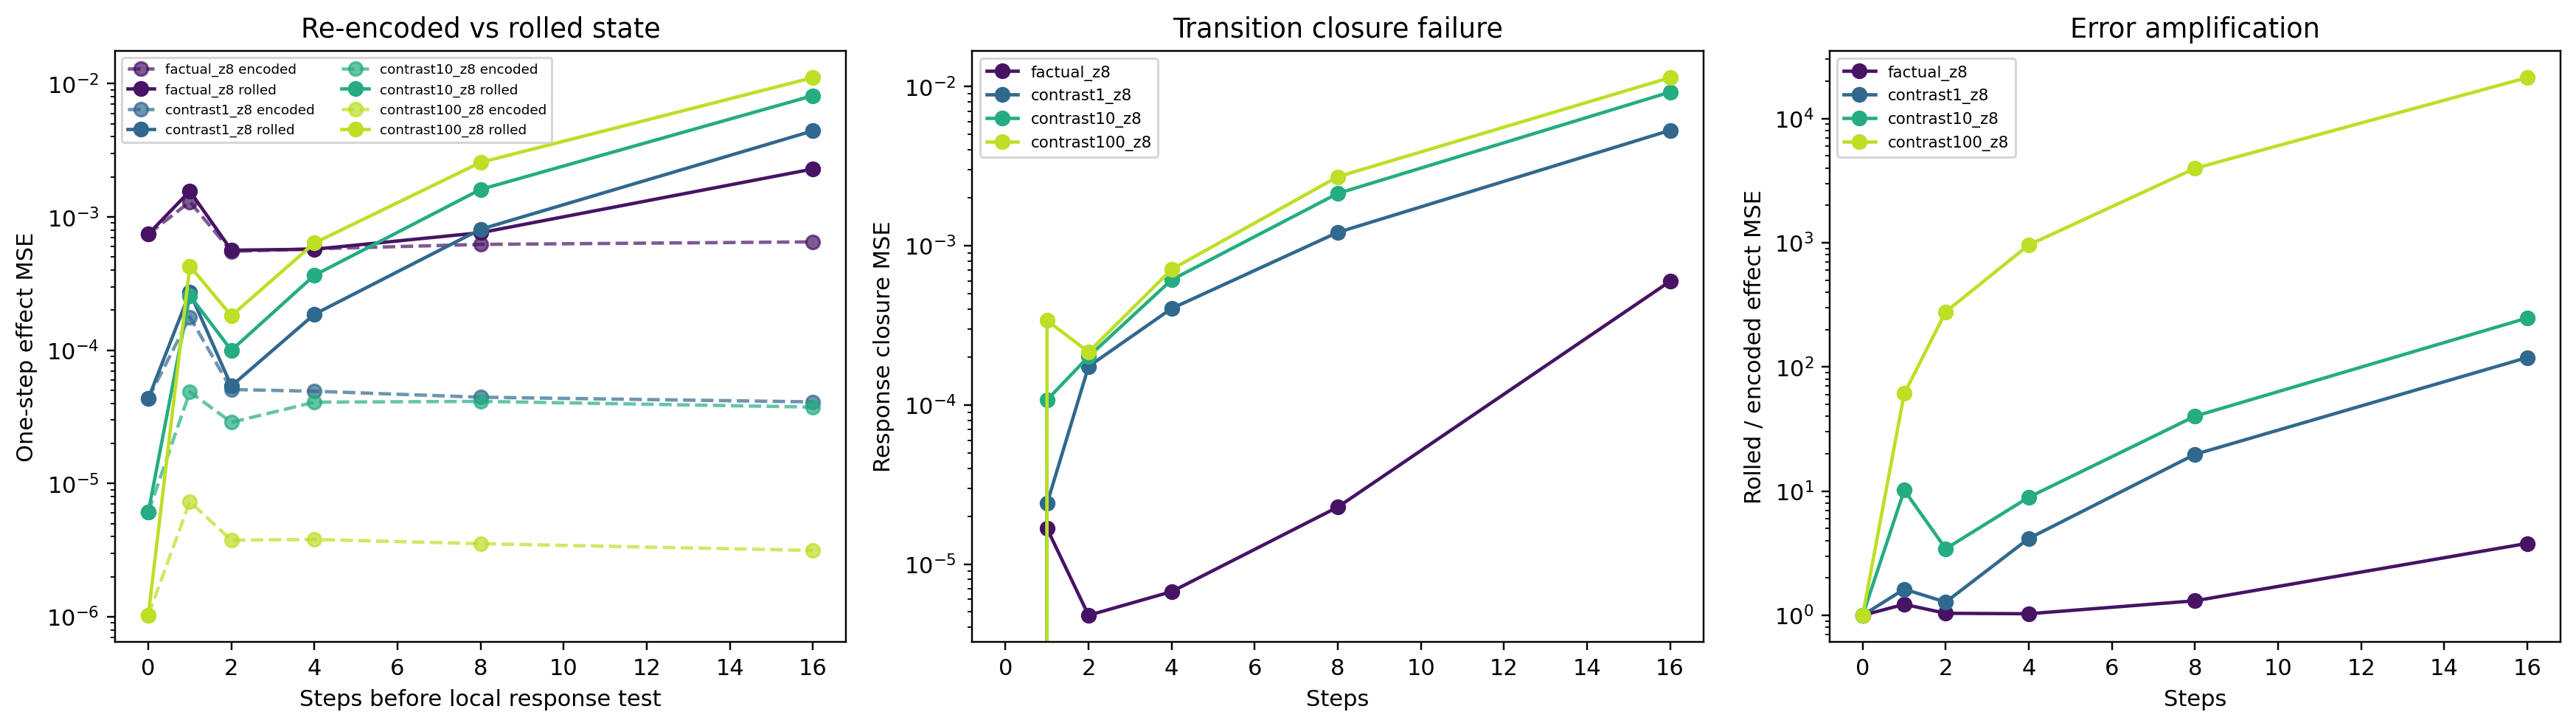
\includegraphics[width=0.97\textwidth]
    {figures/transition_diagnosis/transition_diagnosis.png}
    \caption{Transition diagnosis. Re-encoding the true future history
    can preserve accurate local treatment response even when recursively
    rolled latent states accumulate substantial closure and response
    error. Curves show representative model families; aggregate
    statistics are computed over all 45 fitted models.}
    \label{fig:transition-diagnosis}
\end{figure*}

\subsection{Temporal JEPA Results}
\label{sec:temporal-jepa-results}

We next test whether multi-horizon latent supervision improves 16-step
interventional simulation. Table~\ref{tab:main-results} reports absolute
outcome trajectories, joint observed-state trajectories, and treatment-effect
trajectories on the synthetic interventional test set. All entries are means
with standard errors across five seeds and are multiplied by $10^3$.

\begin{table*}[t]
\centering
\caption{Horizon-16 test performance. Panels A and B report absolute
trajectory MSE under five treatment schedules. Panel C reports treatment-effect
trajectory MSE for each intervention relative to no future treatment. Values
are mean $\pm$ standard error across five seeds, multiplied by $10^3$.
No test metric is used for model selection. Lower is better.}
\label{tab:main-results}
\resizebox{\textwidth}{!}{%
\begin{tabular}{lrrrrr}
\toprule
Method & No treatment & Early block & Alternating & Separated & Late-separated \\
\midrule
\multicolumn{6}{l}{\textit{Panel A: Primary-outcome trajectory MSE, $\mathcal R_X^{(16)}$}} \\
One-step prediction
& $21.648\!\pm\!3.935$ & $40.563\!\pm\!10.499$
& $41.295\!\pm\!9.820$ & $25.829\!\pm\!10.447$
& $21.418\!\pm\!7.570$ \\
Multi-step prediction
& $1.603\!\pm\!0.468$ & $2.676\!\pm\!0.312$
& $1.853\!\pm\!0.113$ & $1.482\!\pm\!0.175$
& $2.020\!\pm\!0.600$ \\
Temporal JEPA ($\lambda_J=1$)
& $\mathbf{0.902}\!\pm\!0.228$ & $\mathbf{1.428}\!\pm\!0.192$
& $\mathbf{1.781}\!\pm\!0.059$ & $\mathbf{1.383}\!\pm\!0.163$
& $\mathbf{1.329}\!\pm\!0.102$ \\
\midrule
\multicolumn{6}{l}{\textit{Panel B: Joint-state trajectory MSE, $\mathcal R_V^{(16)}$}} \\
One-step prediction
& $31.545\!\pm\!4.936$ & $43.701\!\pm\!8.773$
& $42.898\!\pm\!9.747$ & $26.272\!\pm\!7.761$
& $23.955\!\pm\!5.526$ \\
Multi-step prediction
& $1.027\!\pm\!0.247$ & $1.465\!\pm\!0.166$
& $\mathbf{1.028}\!\pm\!0.050$ & $0.833\!\pm\!0.102$
& $1.126\!\pm\!0.328$ \\
Temporal JEPA ($\lambda_J=1$)
& $\mathbf{0.624}\!\pm\!0.170$ & $\mathbf{0.929}\!\pm\!0.088$
& $1.072\!\pm\!0.075$ & $\mathbf{0.805}\!\pm\!0.102$
& $\mathbf{0.769}\!\pm\!0.071$ \\
\midrule
\multicolumn{6}{l}{\textit{Panel C: Treatment-effect trajectory MSE, $\mathcal R_{\mathrm{effect}}^{(16)}$}} \\
One-step prediction
& -- & $30.250\!\pm\!10.087$ & $50.051\!\pm\!17.578$
& $14.974\!\pm\!3.329$ & $7.969\!\pm\!2.120$ \\
Multi-step prediction
& -- & $4.835\!\pm\!0.683$ & $3.238\!\pm\!0.428$
& $1.706\!\pm\!0.296$ & $\mathbf{0.740}\!\pm\!0.091$ \\
Temporal JEPA ($\lambda_J=1$)
& -- & $\mathbf{1.453}\!\pm\!0.269$ & $\mathbf{1.951}\!\pm\!0.258$
& $\mathbf{1.053}\!\pm\!0.058$ & $0.981\!\pm\!0.094$ \\
\bottomrule
\end{tabular}}
\end{table*}

Relative to multi-step prediction, Temporal JEPA reduces mean
$X$-trajectory MSE by $29.2\%$ across all five schedules and improves
every schedule individually. Joint $(X,C)$ trajectory MSE falls by
$23.3\%$ on average and improves on four of five schedules, with a
$4.3\%$ increase under alternating treatment. Mean treatment-effect
trajectory MSE falls by $48.3\%$: JEPA improves early-block, alternating,
and separated effects by $70.0\%$, $39.7\%$, and $38.3\%$, respectively,
but worsens late-separated effect error by $32.7\%$.

Figure~\ref{fig:jepa-main} visualizes the same three test metrics. The
late-separated result highlights that absolute trajectory fidelity and
treatment-effect fidelity are related but non-equivalent: JEPA improves
the absolute $X$ trajectory under this schedule while worsening its
contrast with no treatment.

\begin{figure*}[t]
    \centering
    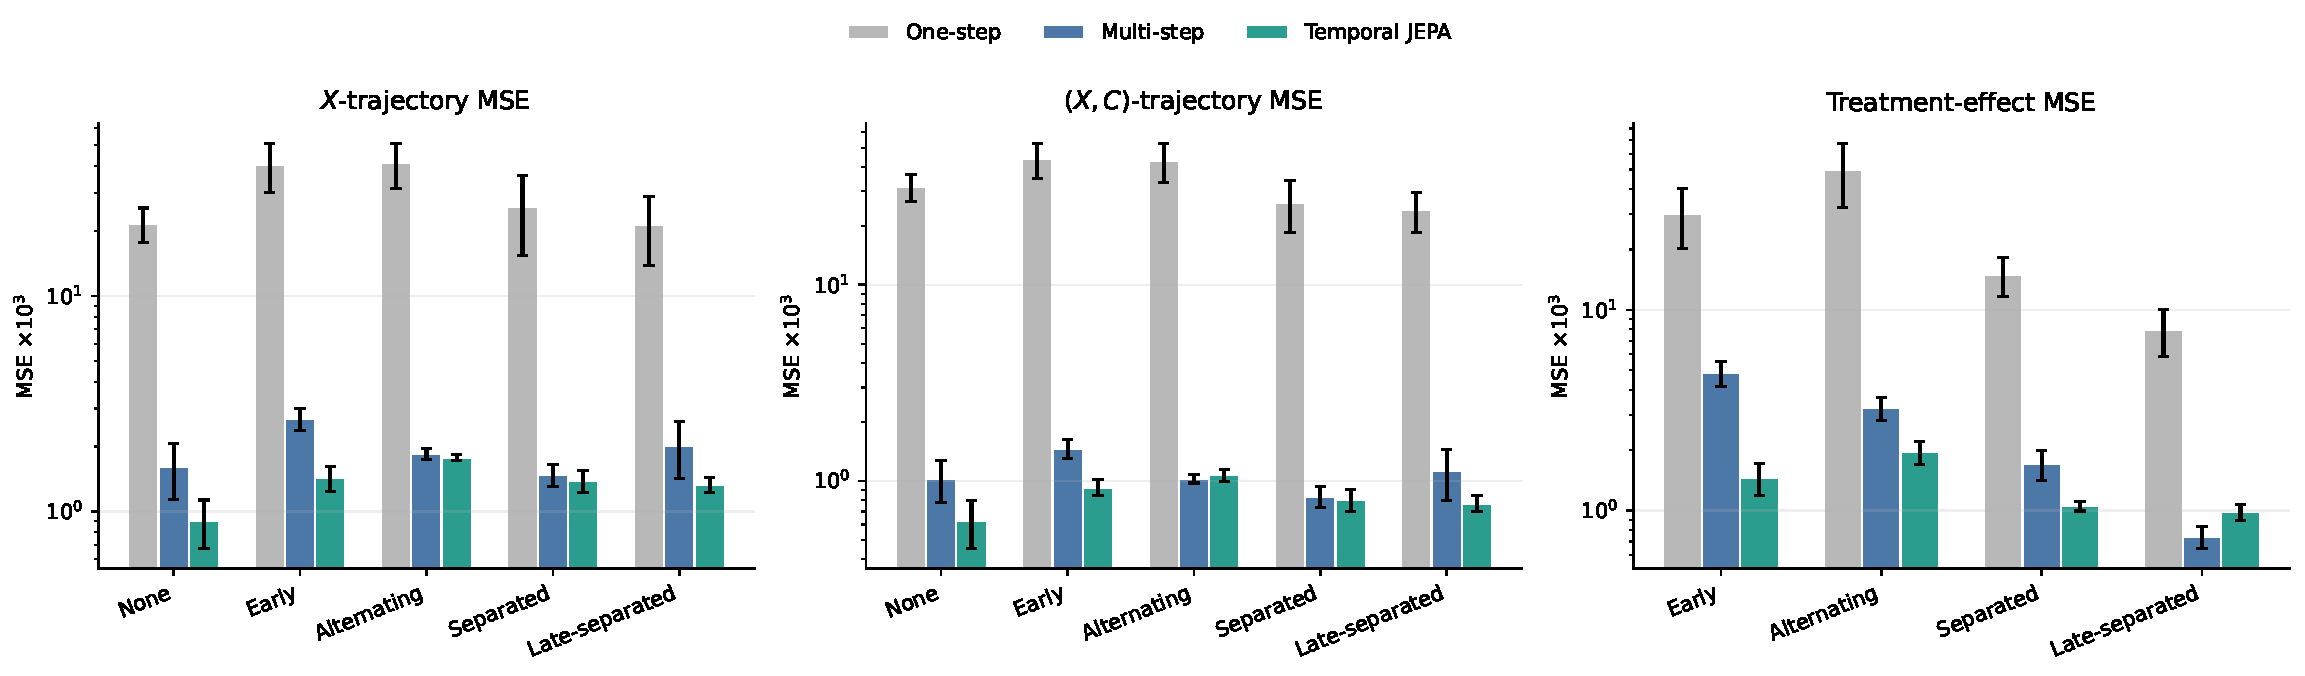
\includegraphics[width=0.97\textwidth]
    {figures/temporal_jepa/interventional_test_metrics.pdf}
    \caption{Horizon-16 synthetic test performance across five seeds.
    Bars show mean MSE and error bars show standard errors. Left:
    primary-outcome trajectory error. Middle: joint $(X,C)$ trajectory
    error. Right: treatment-effect trajectory error relative to no future
    treatment. The vertical axes use logarithmic scales.}
    \label{fig:jepa-main}
\end{figure*}

\subsection{Ablation and Selection Sensitivity}
\label{sec:ablation}

We separate sensitivity of the training design from sensitivity of the
observational selection rule. Full per-schedule and per-seed results are
reported in Appendix~\ref{app:ablation-details}.

\paragraph{Single- versus multi-horizon latent targets.}
We compare JEPA targets at $\{1\}$, $\{8\}$, and
$\{1,2,4,8\}$. Multi-horizon matching reduces horizon-8 closure MSE
from $0.015626$ for one-step JEPA and $0.002437$ for endpoint-only JEPA
to $0.000384$. Their mean horizon-16 effect MSEs across schedules are
$0.001404$, $0.001543$, and $0.001360$, respectively. Multi-horizon
supervision therefore produces the most temporally closed latent
transition, but effect improvement is not monotonic in closure: one-step
JEPA remains competitive on the averaged effect metric.

\paragraph{EMA momentum.}
For multi-horizon JEPA, momentum values $m=0$, $0.9$, $0.99$, and
$0.999$ yield mean horizon-16 effect MSEs of $0.001905$, $0.001289$,
$0.001360$, and $0.001849$, respectively. Moderate target smoothing is
beneficial, but larger momentum is not monotonically better. We retain
the prespecified $m=0.99$ for the main comparison rather than retuning
the reported method on counterfactual test performance.

\paragraph{JEPA weight and observational selection.}
We train $\lambda_J\in\{0.1,1,10\}$. Increasing $\lambda_J$ lowers
closure error but eventually violates the factual prediction gate. At
the prespecified gate $\gamma=1.10$, selection horizons
$H_c\in\{2,4,8\}$ all choose $\lambda_J=1$. The selected weight is,
however, sensitive to the factual-fidelity tolerance: at $H_c=8$,
$\gamma=1.05$, $1.10$, and $1.20$ select $\lambda_J=0.1$, $1$, and
$10$, respectively, while no JEPA candidate satisfies the strict
$\gamma=1.00$ gate. The tolerance is therefore a substantive trade-off,
not an innocuous constant.

\subsection{Summary of Findings}

The experiments support three conclusions. First, factual prediction can
conceal both loss and incorrect propagation of treatment-relevant
information. Second, Temporal JEPA can improve latent transition
consistency and long-horizon treatment-effect estimation without a large
loss of factual fidelity. Third, neither latent closure nor a particular
training design is sufficient to guarantee effect accuracy across all
treatment timings. These findings support latent temporal consistency as
a useful complementary diagnostic and learning signal, rather than a
standalone certificate of causally valid simulation.
